\section{Цель работы}
	Описать сценарии, которые реализует система.
\section{Порядок выполенения работы}
	\subsection{Диаграмма деятельности}
	
		Диаграмма деятельности для всей системы указана на рис. 1.
	
		\begin{figure}[ht] 
			\center
			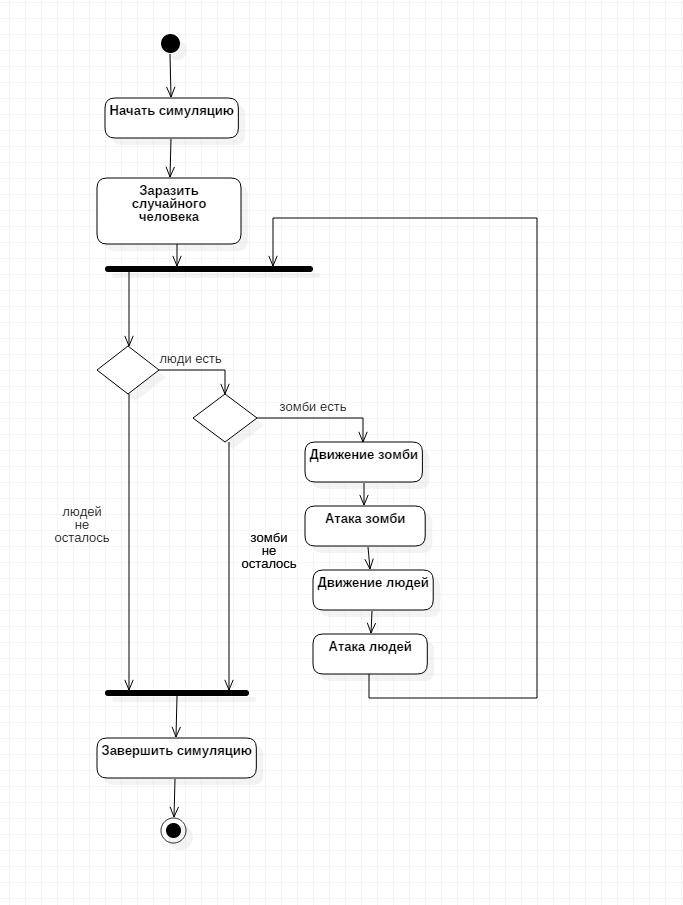
\includegraphics [width=0.6\textwidth] {UML-activity.png}
			\caption{Диаграмма деятельности} 
		\end{figure}
		\FloatBarrier
		\clearpage
	%\subsection{Диаграмма прецедентов}
		
	\subsection{Последовательность действий}
	
	Последовательность действий изложена в терминах FIPA-протоколов.
	
	В системе есть управляющий агент, который занимается рассылкой сообщений о том, что начался очередной ход (ход движения зомби, ход атаки людей и т.д.).
	
	В начальный момент времени он ждёт, пока не появится необходимое количество агентов, которые получают у него начальные данные по протоколу \textbf{Query-ref} (размер карты, их координаты, сгенерированные случайно). В конце случайно выбирается первый агент-заражённый, все остальные - люди.
		
	Далее агент управляющий полчает всех агентов нужного типа (зомби/человек) в жёлтой книге (DFService). Всем им отправляется \textbf{Request} соответствующего текущей стадии симуляции действия. Это повторяется, пока все объекты в системе не станут одного типа.
	
	\subsubsection{Движение}
		Участник отправляет всем людям запрос всем соперникам \textbf{Query-ref} об их координах в определённом радиусе от него. Соперники вне радиуса отвечают отказом, а соперники в заданном радиусе передают координаты.
		
		Далее ходячий двигается в зависимости от своей текущей роли и состояния.
		
	\subsubsection{Атака}
		Участник отправляет запрос \textbf{Query-ref} всем соперникам о нахождении в той же точке, что и он. Далее происходит атака одного из найденных соперников, если таковые есть.